%%%%%%%%%%%%%%%%%%%%%%%%%%%%%%%%%%%%%%%%%%%%%%%%%%%%%%%%%%%%%%%%%%%%%%%%%%%
%% This file is part of the book
%%
%% Algorithmic Graph Theory
%% http://code.google.com/p/graph-theory-algorithms-book/
%%
%% Copyright (C) 2009--2011 Minh Van Nguyen <nguyenminh2@gmail.com>
%%
%% See the file COPYING for copying conditions.
%%%%%%%%%%%%%%%%%%%%%%%%%%%%%%%%%%%%%%%%%%%%%%%%%%%%%%%%%%%%%%%%%%%%%%%%%%%

\documentclass{article}

\usepackage{tikz}
\usepackage{tkz-berge}  %% for drawing combinatorial graphs
\usetikzlibrary{external}
\tikzexternalize{weighted-Chvatal-graph}

\begin{document}

\begin{figure}
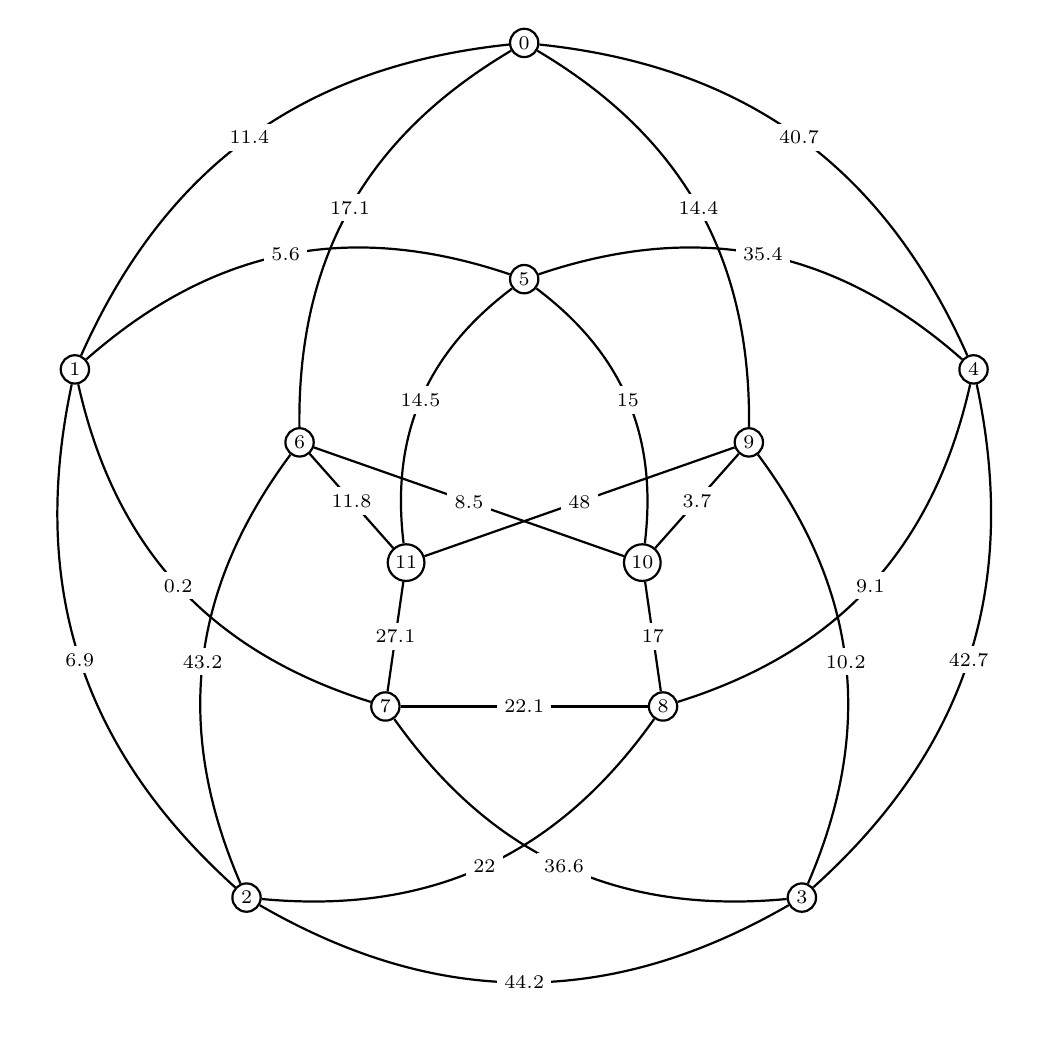
\begin{tikzpicture}
[lineDecorate/.style={-,thick},%
  nodeDecorate/.style={shape=circle,inner sep=1.5pt,draw,thick},%
  scale=3]
\scriptsize
%% nodes or vertices
\foreach \nodename/\x/\y in {
  %% inner star
  5/0.0/1.0, 9/0.9510/0.3090, 8/0.5877/-0.8090, 7/-0.5877/-0.8090,
  6/-0.9510/0.3090,
  %% outer pentagon
  0/0.0/2.0, 4/1.9021/0.6180, 3/1.1755/-1.6180, 2/-1.1755/-1.6180,
  1/-1.9021/0.6180,
  %% inner two nodes
  10/0.5/-0.2, 11/-0.5/-0.2}
{
  \node (\nodename) at (\x,\y) [nodeDecorate] {\scriptsize$\nodename$};
}
%% edges or lines
\tikzstyle{EdgeStyle}=[-,thick]
\tikzstyle{LabelStyle}=[fill=white]
\foreach \startnode/\endnode/\bend/\weight in {
  0/1/bend right/11.4, 0/4/bend left/40.7, 0/6/bend right/17.1,
  0/9/bend left/14.4, 1/2/bend right/6.9, 1/5/bend left/5.6,
  1/7/bend right/0.2, 2/3/bend right/44.2, 2/6/bend left/43.2,
  2/8/bend right/22, 3/4/bend right/42.7, 3/7/bend left/36.6,
  3/9/bend right/10.2, 4/5/bend right/35.4, 4/8/bend left/9.1,
  5/10/bend left/15, 5/11/bend right/14.5, 6/10/bend left=0/8.5,
  6/11/bend left=0/11.8, 7/8/bend left=0/22.1, 7/11/bend left=0/27.1,
  8/10/bend left=0/17, 9/10/bend left=0/3.7, 9/11/bend left=0/48}
{
  \Edge[label=$\weight$,style=\bend](\startnode)(\endnode)
}
\end{tikzpicture}
\end{figure}

\end{document}
